\section{Relevant Results from Prior NSF Support}
\noindent {\bf Rolf Ryham}: no prior NSF support.

\noindent
{\bf Yuan-Nan Young}: {\em NSF-DMS-1222550, Mathematical and
experimental study of lipid bilayer shape and dynamics mediated by
surfactants and proteins}, \$212,603, 9/15/2012 - 08/31/2016 (with
no-cost extension), PI. {\em Intellectual merit:} The focus of this
grant is modeling the interaction between a pure lipid bilayer membrane
with surfactant, cholesterol, and protein.

\noindent
{\it Broader impacts:} 
One PhD student (Szu-Pei Fu) was funded to work with PI Young, and work
has resulted in seven papers~\cite{Nganguia2013_PoF, Nganguia2013_PRE,
Young2014_JFM, Young2015_PoF, Nganguia2015_CiCP, Pak2015_PNAS,
fu2015pre}. PI Young has been actively involved with promotion of
underrepresented students at NJIT. One PhD student, Herve Nganguia, is
now an Assistant Professor at Towson University. PI Young has taught a
broad spectrum of courses in fluid mechanics and applied math modeling.

\noindent
{\bf Bryan Quaife}: {\em NSF DMS-2012560, Erosion, Transport, and
Dispersion in Granular and Porous Media}, \$249,636,
08/01/2020--07/31/2023, PI. {\em Intellectual Merit:} The goal of this
research is to develop high-order numerical methods to
simulate hydrological processes including erosion.

\noindent
{\it Broader impacts:} 
A third-year PhD student (Jake Cherry) has been assigned to this
project. One paper has been accepted~\cite{che-lin-her-qua2022} and
another is under review~\cite{moo-che-chi-qua2022}.

\section{Project Management, Collaboration Plan, and Schedules of
Research Tasks}
\setlength{\parindent}{0pt}
% N.B. wrapfigure is not compatible with \noindent.

\begin{wrapfigure}[10]{r}{0.4\textwidth}
  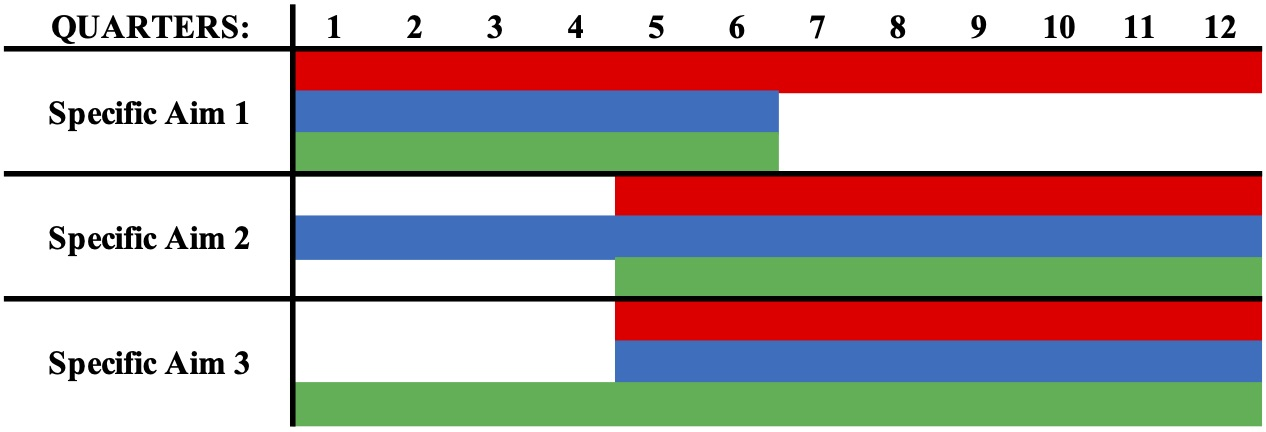
\includegraphics[width=0.4\textwidth]{figures/gantt.jpg}
  \caption{\label{fig:schedule} Schedule for the proposed work, measured
  in quarters from the beginning of the project. The lead PI of each
  Specific Aim will be Ryham (red), Quaife (blue), and Young (green).}
\end{wrapfigure}


\begin{comment}
\begin{wrapfigure}[11]{r}{0.56\textwidth}
\vspace{-19pt}
%\definecolor{barblue}{RGB}{51,102,254}
%\renewcommand\sfdefault{phv}
%\renewcommand\mddefault{mc}
%\renewcommand\bfdefault{bc}
%\sffamily
\begin{ganttchart}[
    canvas/.append style={fill=none, draw=black!5, line width=.75pt},
        x unit =4.5mm,
        y unit chart =\baselineskip,
    hgrid style/.style={draw=black!5, line width=.75pt},
    vgrid={*1{draw=black!5, line width=.75pt}},
    title/.style={draw=none, fill=none},
    title label font=\bfseries\footnotesize, % numbers across the top
    title label node/.append style={below=3pt},
    include title in canvas=false,
    bar label font=\mdseries\footnotesize\color{black!70}, 
    % titles across the left
    %bar label node/.append style={left=2cm},
    bar/.append style={draw=none, fill=blue},
    bar incomplete/.append style={fill=blue},
    bar progress label font=\mdseries\footnotesize\color{black!70},
    milestone label font=\mdseries\small\color{black!70},
        milestone left shift =0.9,
        milestone right shift =0.1,
        % Don't draw group bars
        group height =0,
        group peaks height =0,
        group label font =\bfseries\small,
]{1}{12}
\gantttitle[
    title label node/.append style={below left=3pt and -6pt}
]{QUARTERS:\quad1}{1}
\gantttitlelist{2,...,12}{1} \\
%\ganttgroup{Tasks\hfill}{1}{12}\\
\ganttbar[bar/.append style={fill=red}]{Specific Aim 1}{1}{12} \\
\ganttbar[bar/.append style={fill=blue}]{Specific Aim 2}{1}{12}\\
\ganttbar[bar/.append style={fill=green}]{Specific Aim 3}{1}{12}\\
\ganttbar[bar/.append style={fill=black}]{Program Management}{1}{12}
\ganttbar[bar/.append style={fill=magenta}]{}{4}{4}
\ganttbar[bar/.append style={fill=magenta}]{}{8}{8}
\ganttbar[bar/.append style={fill=magenta}]{}{12}{12}
\end{ganttchart}
\vspace{-10pt}
\caption{Schedule for the proposed work, measured in quarters from the
  beginning of the project. The lead PI of each Specific Aim will be
  Ryham (red), Quaife (blue), and Young (green). Project management will
  be continuous (black), but we anticipate extra attention will be
  necessary to align objectives in quarters 4, 8, and 12 (magenta).}
\label{fig:schedule}
\end{wrapfigure}
\end{comment}
\textbf{Project management}: 
%
The success of the proposed research requires complementary expertise
and collaborative efforts in physics, applied mathematics, algorithms,
and computing. PI Ryham has been working on mathematical modeling with a
strong analytical background. PI Young has been working on many areas of
computational fluid dynamics and applications to math biology for many
years. PI Quaife has been working on integral equation methods, fast
algorithms, and their applications to fluid dynamics for many years.
Their recent collaborative works on the granule-based vesicles in two
dimensions~\cite{FuQuRyYo22, fu-ryh-qua-you2022} has provided a solid
foundation for the proposed research.

\smallskip

\textbf{Collaboration plan}: 
%
The management responsibility of this collaborative research will reside
with the lead PI (Quaife) for this endeavor. The research work is
structured to meet the tasks discussed in \S\ref{sec:proposed-work}. The
PIs and students will meet frequently on Zoom and in person when
possible. PI Ryham and PI Young will conduct biweekly meetings in
person, with PI Quaife Zoom in from Florida. The PIs will share software
packages, paper sources, and references on a common \textsf{Git}
repository. The resulting software packages will be posted on the
\textsf{Github} software repository.
%
%\smallskip
%
\textbf{Research Schedule:} The detailed schedule for the proposed work
is shown in Figure~\ref{fig:schedule}. Each PI will spearhead a
different Specific Aim, and program management will happen
throughout, with special coordination taken in quarters 4, 8, and
12.


